\chapter{NLOS measurements results}

The \gls{csi} processing approaches and radar algorithms presented in the previous sections were evaluated with real measurements obtained using Nokia's ISAC FR2 prototype described in Section \ref{sec:intro-PoCarchitecture}.

\section{Measurements setup}
\label{sec:Test1_meas_scenario}

The system was mounted in an indoor industrial test facility, with gNB and sniffer positioned at a height of $5.12$ m. The transmitter was oriented towards a wide  indoor area free of obstacles. The antenna pole was located approximately 23 metres from a warehouse rack (installed in front of a concrete wall) and a cargo door.
Figure \ref{fig:Test1_arena_plan} shows a scheme of the test area layout.

The observed measurement area was free of any major obstructions or occlusions that could be used to create a \gls{nlos} scenario under normal conditions.
Nonetheless, it was possible to generate \gls{nlos} conditions by directing the signal over the target and towards the wall, observing the reflected returns.

 
The tests were carried out using:

\begin{enumerate}
	\item A human target.
	\item A strong reflector (large metal cabinet with flat surfaces).
\end{enumerate}

The direction (azimuth $\theta$ and elevation $\varphi$) of the transmitted and received beams (\ie of the \gls{gnb} and of the sniffer) was fixed for the whole measurement.
Before each test, a short calibration measure is performed, which includes only the static elements of the scenario. The calibration data will be used in the post-processing steps for clutter removal as described in Section \ref{sec:clutter_removal}.

\begin{figure}[H]
	\centering
	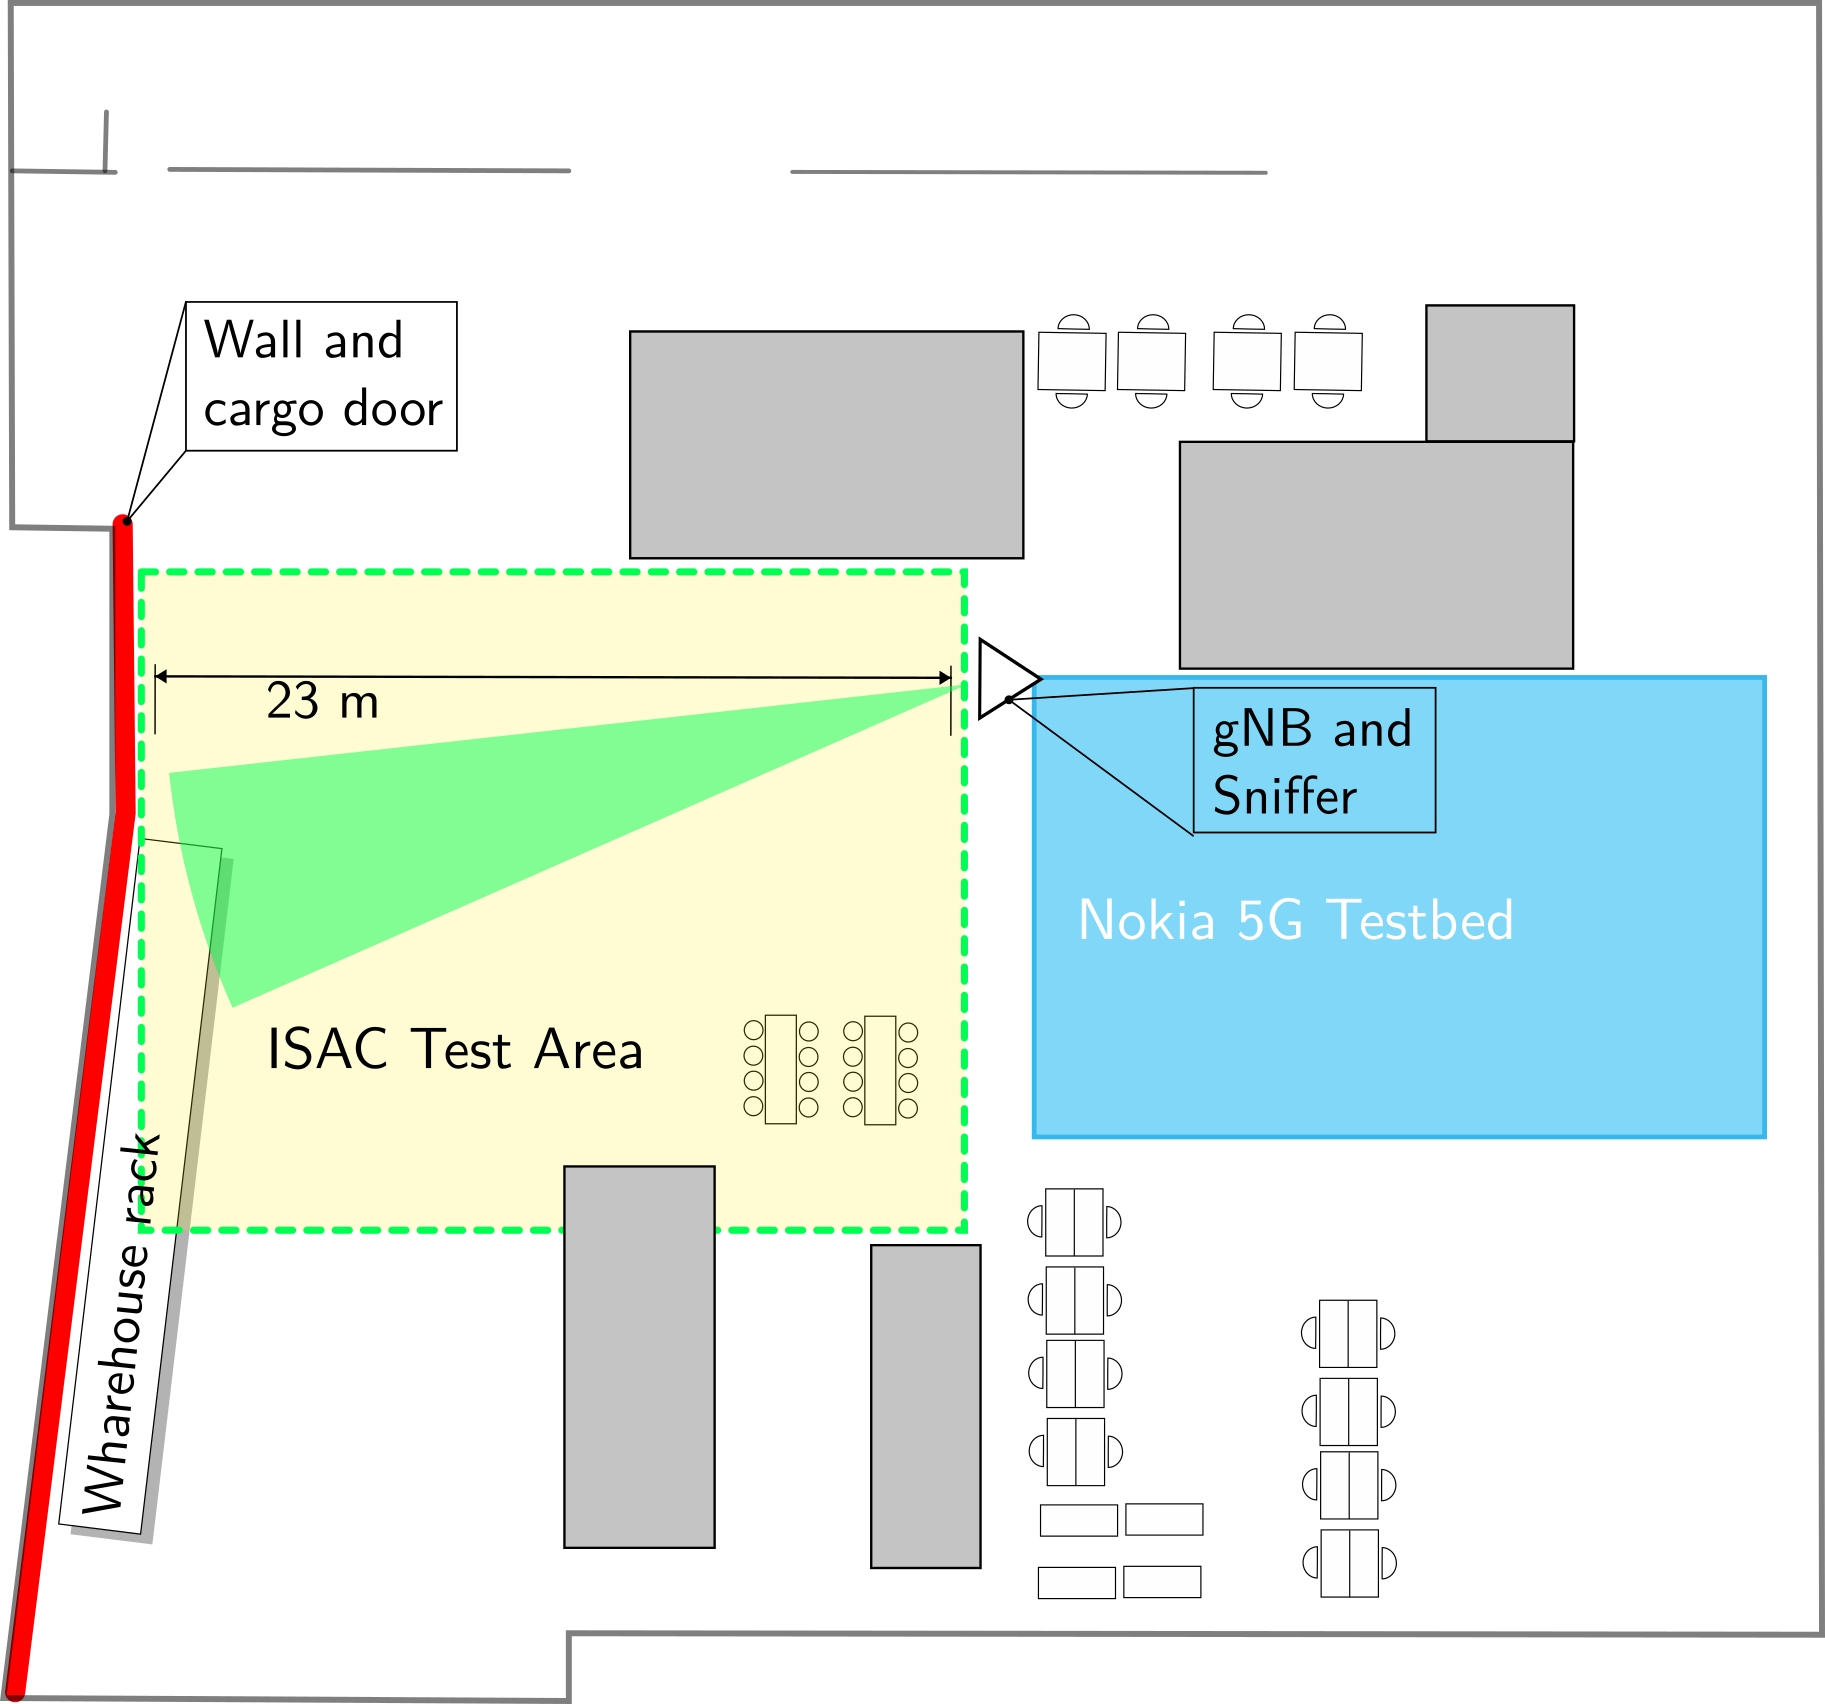
\includegraphics[width=.6\textwidth]{Images/Test1/arena_plan}
	\caption{Scheme of the PoC deployment layout in ARENA 2036, Stuttgart.}
	\label{fig:Test1_arena_plan}
\end{figure}


\section{Measurement Scope: Detection Rate}

The radar system using OFDM can determine the range and radial speed of a target (this experiment used a fixed beam, hence the \gls{aoa} was considered constant). If an object moves tangentially \wrt the sensing system, it will appear as static.
The test aimed to maximize the radial speed of the target to analyse the characteristics of the signal generated by its reflection off the wall.
In plausible intrusion detection scenarios, it can be assumed that an eventual intruder will move within the surveilled area at some point., allowing to leverage its Doppler component for detection (and separation from static clutter).

During the initial measurement, the antenna boresight was directed perpendicular to the wall, with null azimuth $\theta$.
The target moved radially between the transmitter and reflector. The test subject moved towards the \gls{gnb} and back multiple times in a straight line during the measurements.
Due to the rather large beamwidth of the system, $\pm$7\textdegree\hspace{1pt} in azimuth and elevation, and its sidelobes, both \gls{los} and \gls{nlos} components can be jointly observed in our measurements, as shown in Figure \ref{fig:Test1_base-lateral_view}.

During the measurement, the direct component was always visible as no other obstacle was positioned in the scene. 
The observed \gls{los} component is critical for this study, as it represented a source of ground truth and can be used as a correct estimate of the target's position in the test area.
It must be noted that this additional information does not have any bearings on the \gls{nlos} detection capabilities of the sensing setup, but it's used, given 
the knowledge of the geometry of the test area, to obtain an estimate of the position and velocity of the NLOS return. 

\begin{figure}[H]
	\centering
	
	\subfloat[\small Lateral view of measurement scenario. NLOS return (red) is coupled with a LOS component (orange) generated from the secondary lobe.
	\label{fig:Test1_base-lateral_view}]{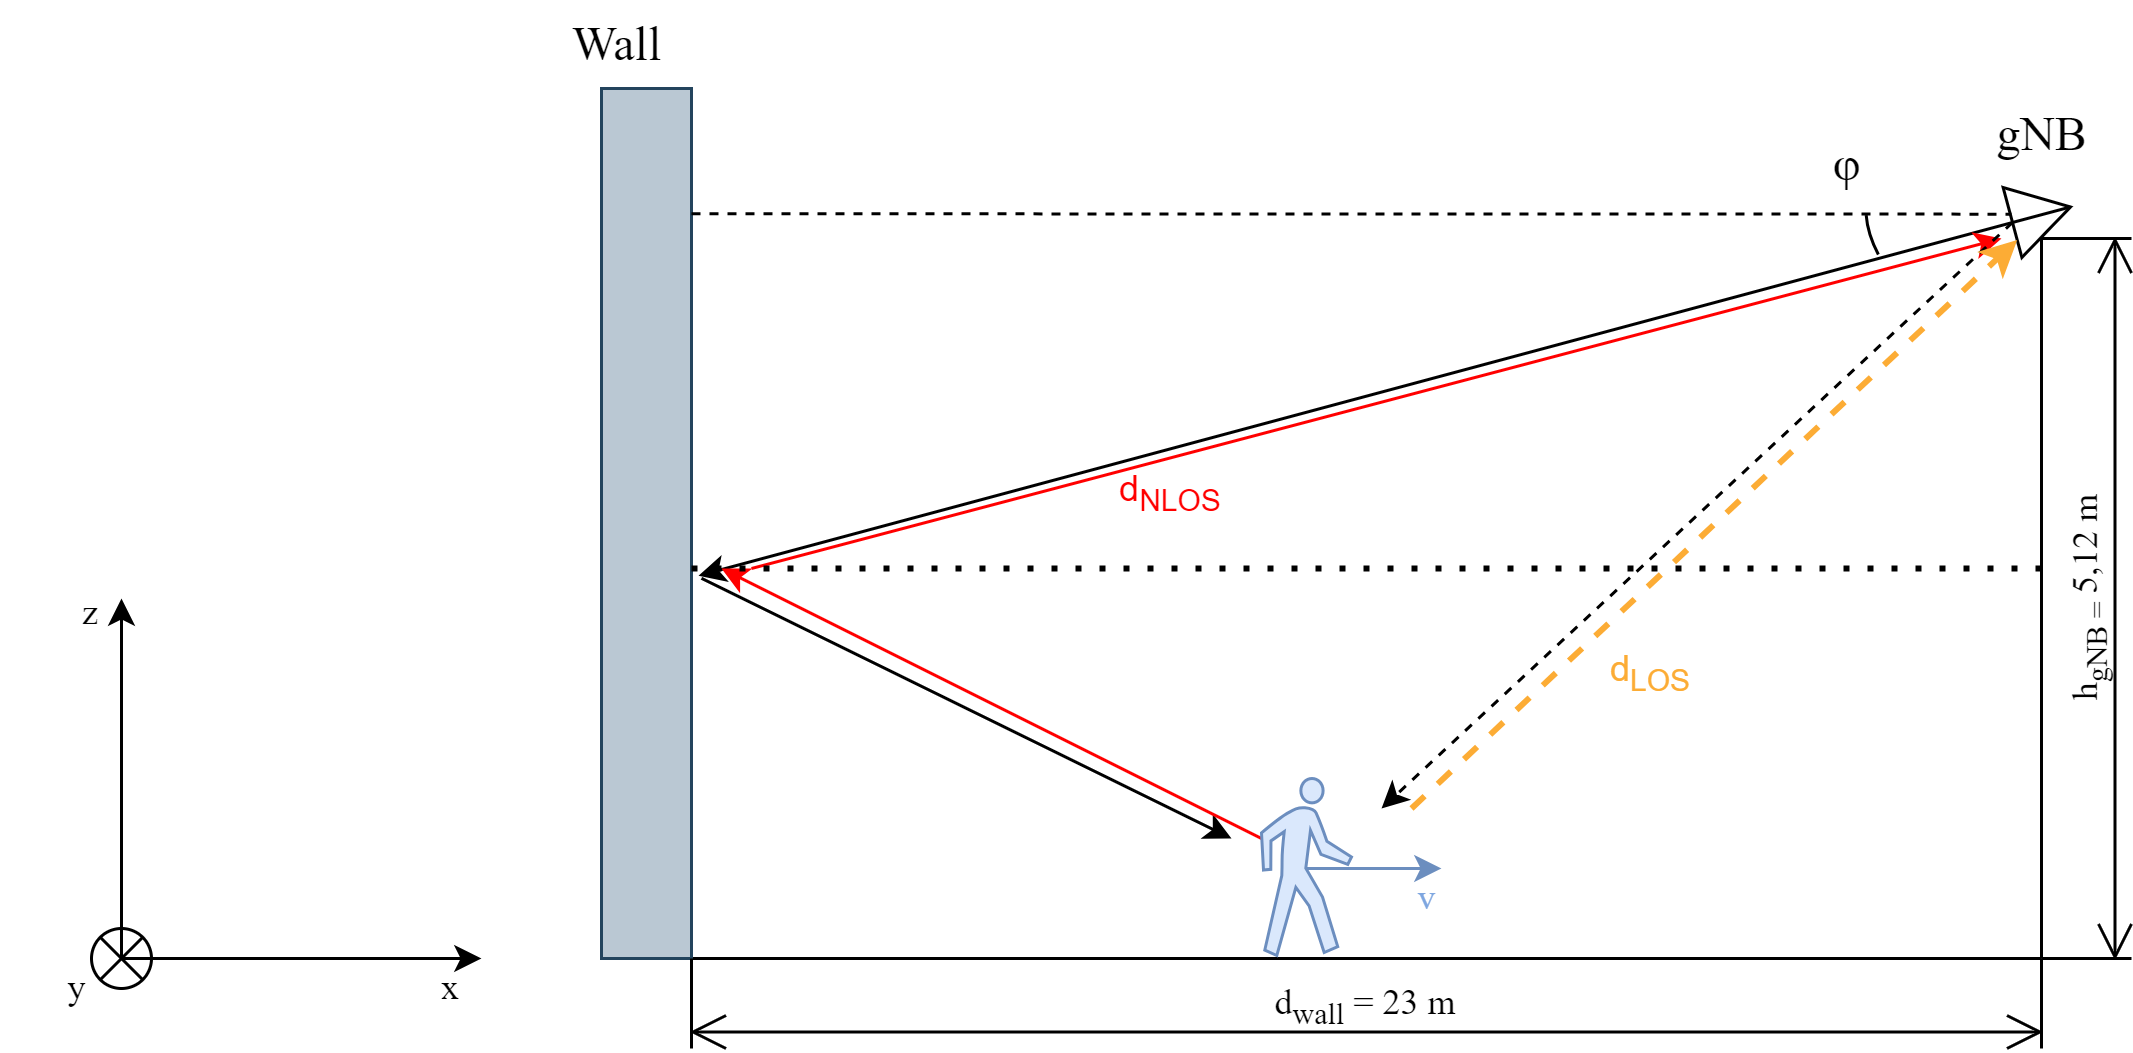
\includegraphics[width=1\textwidth]{Images/Test1/base-lateral_view_los_geometry}
	}
	\\
	\subfloat[\small Top view of measurement scenario. \label{fig:Test1_base-top_view}]{
		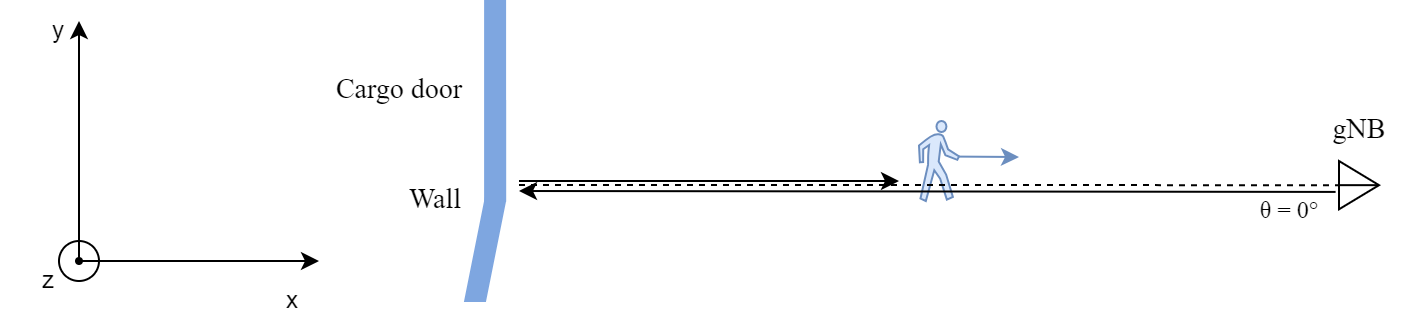
\includegraphics[width=1\textwidth]{Images/Test1/base-top_view}
	}
	\caption{Scheme of the measurement scenario}
	\label{fig:Test1_base_and_top_view}
\end{figure}

Considering the processing scheme proposed in Section \ref{sec:nlos_proc_pipeline}, the periodogram was processed differently after separation in the regions corresponding to LOS and NLOS conditions. A visual example of the separation between the two regions was presented in Figure \ref{fig:Rad_nlos_los_separation}.
A standard strongest peak search was performed for the LOS region, while multiple peak detection was conducted in NLOS. This assumption was made since the test was conducted in a single target scenario and a single moving target in \gls{los} is expected.
Accurate range and velocity measurements are obtained after interpolation of each peak with the adjacent bins.

In order to make use of the \gls{los} return, its speed and range values were used to validate if any \gls{nlos} peak corresponds with a target.
The expected range and speed values of the \gls{nlos} return were estimated as:

\begin{itemize}
	\item Expected speed:
	$$ \hat{v}_{\text{NLOS}} = -v_{\text{LOS}}$$
	direct and reflected beams will hit the target from the opposite direction, hence measuring the target's speed with opposing sign.
	\item Expected range, estimated considering the model in Figure \ref{fig:Test1_base-lateral_view} as:
	$$ \hat{d}_{\text{NLOS}} = 2 d_{\text{wall}} - d_{\text{LOS}}\cdot \cos{\left(\arctan{\left(\frac{h_{\text{gNB}}}{d_{\text{LOS}}}\right)}\right)}$$
\end{itemize}

The two estimated values were used to determine if any of the detected \gls{nlos} peaks corresponded with the target.

\textit{Detection rate} was defined as the metric used to evaluate the experiment: at each update, if the speed and range of the NLOS return matched the expected values calculated from the LOS data ($d_{\text{NLOS}} \approx  \hat{d}_{\text{NLOS}}$ and $v_{\text{NLOS}} \approx \hat{v}_{\text{NLOS}}$), detection was considered positive.
The detection rate was then obtained as the ratio between the number of updates in which the NLOS component was above threshold, and the total number of updates in which the LOS component was detected.


\begin{equation*}
	\text{Detection rate} = \frac{\text{updates with NLOS}}{\text{updates with LOS}}
\end{equation*}

Due to the multiple reflections, the NLOS return presented considerably smaller power compared to LOS.
This meant that due to the presence of large clutter returns and their sidelobes, this return is not necessarily the strongest one in the NLOS region of the periodogram.
The five strongest detected peaks in \gls{nlos} were considered and detection rate evaluated based on whether one of those peaks corresponded with the \gls{nlos} return.
\section{Evaluation on detection rate of a strong reflector}

	\begin{figure}[H]
	\centering
	
	\subfloat[\footnotesize Metal cabinet moving towards gNB, linear scale.\label{fig:Test1_metal_lin}]{%
		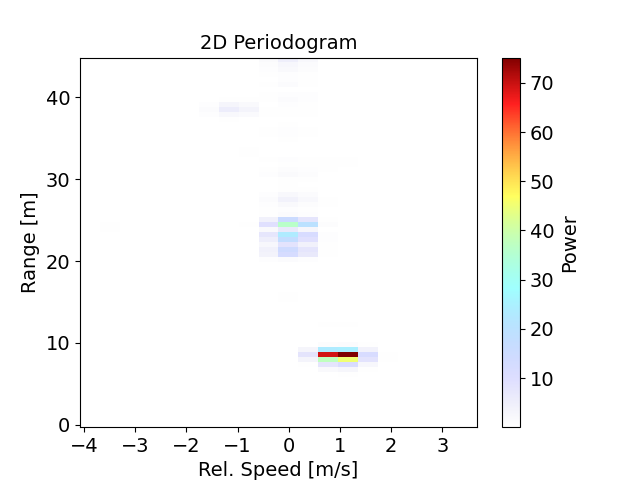
\includegraphics[scale=0.45]{Images/Test1/per_strong_ref/linear_1frame_dec_CRAP.png}%
	}\hfill
	\subfloat[\footnotesize Metal cabinet moving towards gNB, power in dB.\label{fig:Test1_metal_db}]{%
		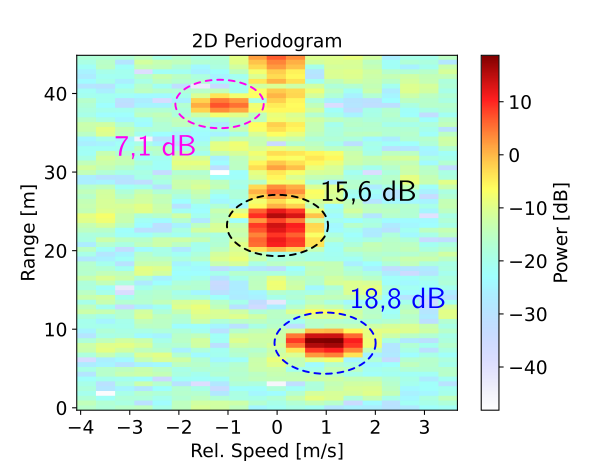
\includegraphics[scale=0.45]{Images/Test1/per_strong_ref/db_1frame_dec_CRAP_labelled_text22.png}%
	}\hfill
	\subfloat[\footnotesize Human target walking towards gNB, power in dB.\label{fig:Test1_metal_human-baseline}]{
		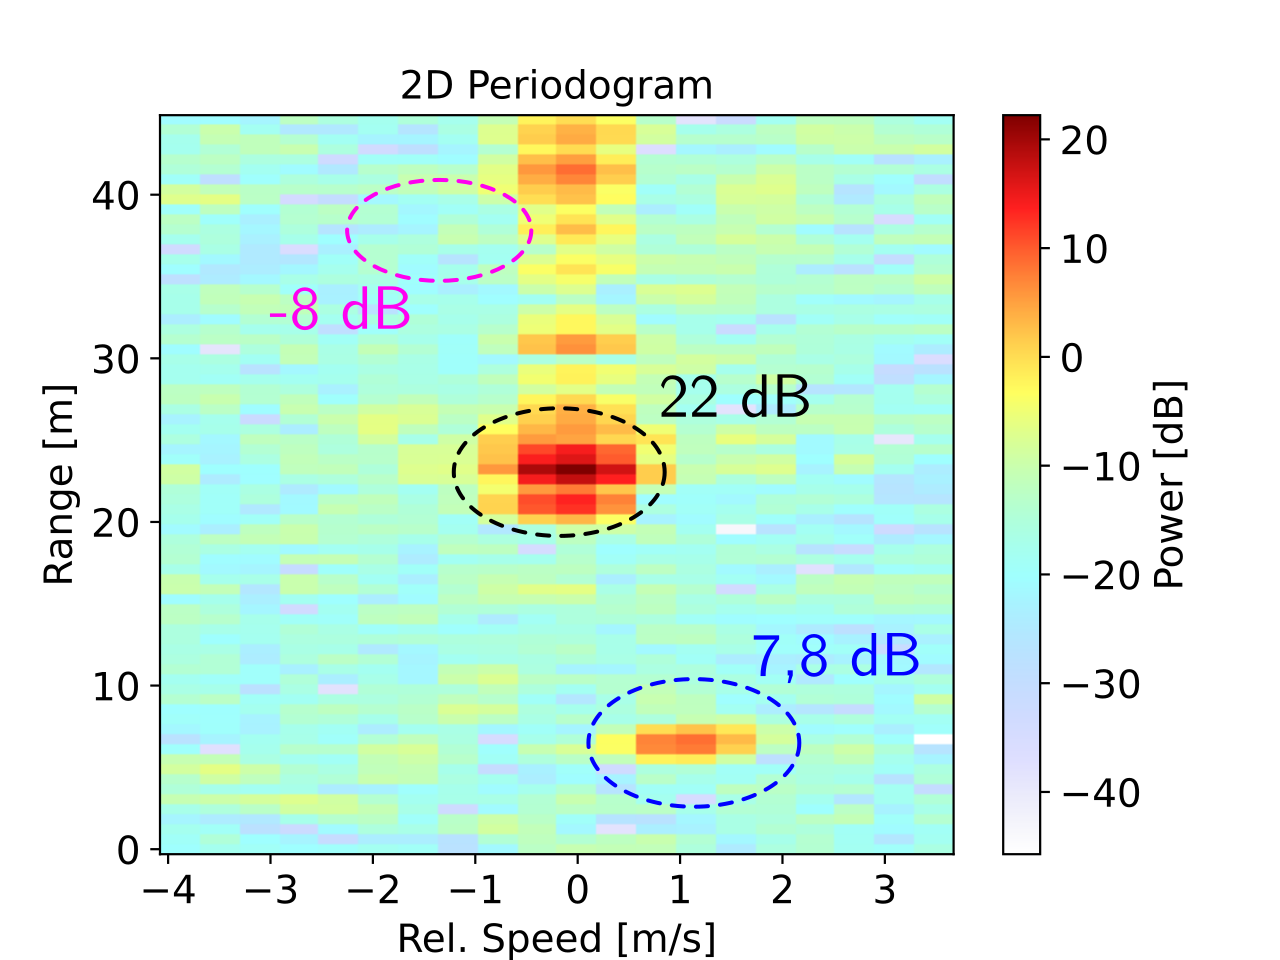
\includegraphics[scale=0.45]{Images/Test1/per_strong_ref/db_1frame_dec_CRAP_HUMAN_labelled_text22.png}
	}
	\caption[]{\small Comparison of periodograms from sensing acquisitions obtained in NOKIA's industrial test facility.
		All the periodograms are obtained by processing a single decimated CSI frame (24 symbols), after applying clutter removal with CRAP.
		Periodograms \subref{fig:Test1_metal_lin} and \subref{fig:Test1_metal_db} show the returns obtained with the metal cabinet. All the periodograms contain three returns: one from the wall at 23 m (black) and two from the moving targets, one from LOS (blue) and the other from NLOS (purple). The NLOS return is clearly separated from the underlying noise floor, even when processing only 24 symbols. On the contrary the NLOS component generated from the human target in \subref{fig:Test1_metal_human-baseline}, requires for a considerably higher processing gain to be detected reliably.}
	\label{fig:Test1_metal-human_comparison}
	\end{figure}
The first measurement was performed with the strong reflector, which represented an ideal scenario. 
Figure \ref{fig:Test1_metal-human_comparison} illustrates the comparison between the human and the metal cabinet cases. 
Even when decimating the single \gls{csi} matrix, with a 15 dB loss in processing gain, the NLOS component of the metal cabinet can be easily identified when moving.
The detection rate test displayed in figure \ref{fig:Test1_detect_rate_strong_ref} shows that the passive reflector, thanks to its significantly larger radar cross section, is clearly identified while it is moving and has stronger power compared to reflected clutter returns.
\begin{figure}[H]
	\centering
	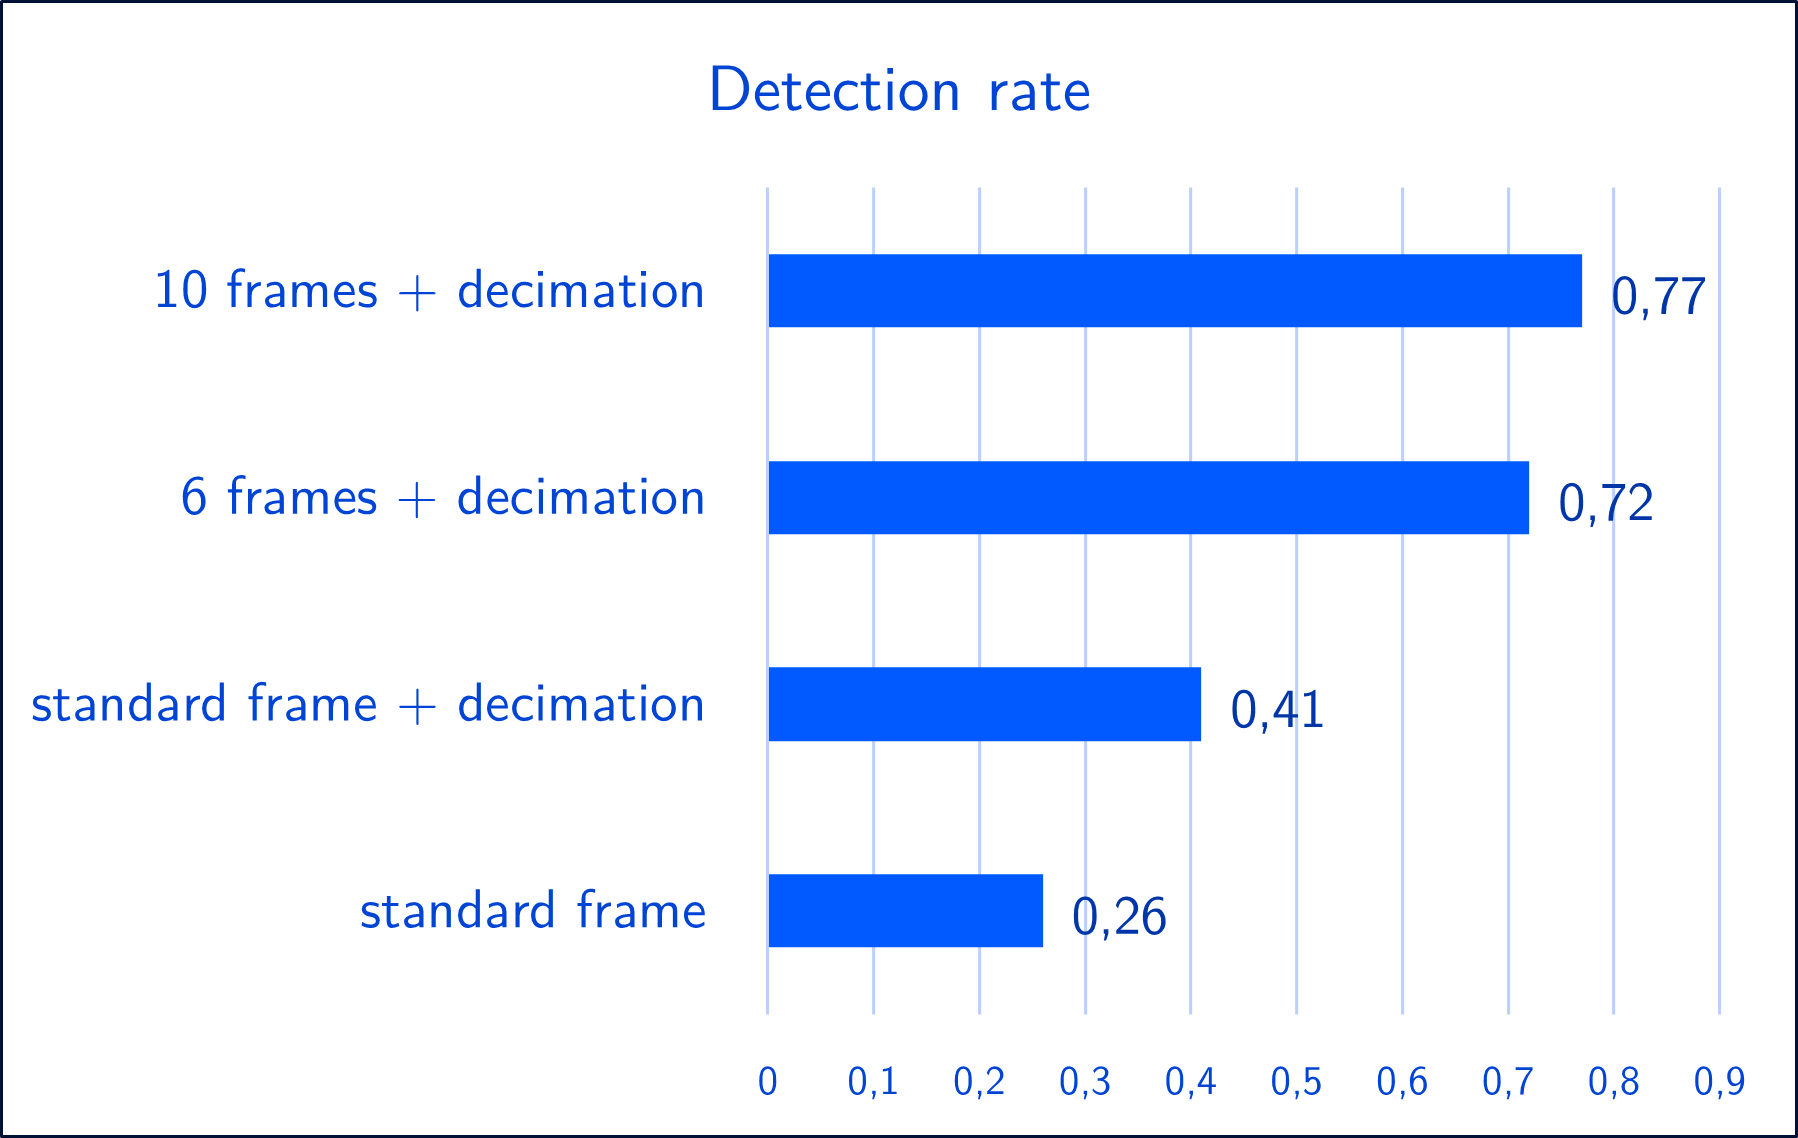
\includegraphics[width=0.7\textwidth]{Images/Test1/detect_hist/detect_hist_cabinet_LMsans.png}
	\caption{\small Detection rate observed for passive metal reflector target in mixed LOS/NLOS measurement.}
	\label{fig:Test1_detect_rate_strong_ref}
\end{figure}
Passing the NLOS measurements to a Kalman filter it was possible to track the target in the range/Doppler plane, as shown in figure \ref{fig:Test1_kf_track_strong_ref}. This result is to show that one of the main limitation of NLOS signals is the strength of the target return. Objects with large \gls{rcs} are easier to separate from the noisy background and the effect of fading and obstruction is relatively small.
\begin{figure}[H]
	\centering
	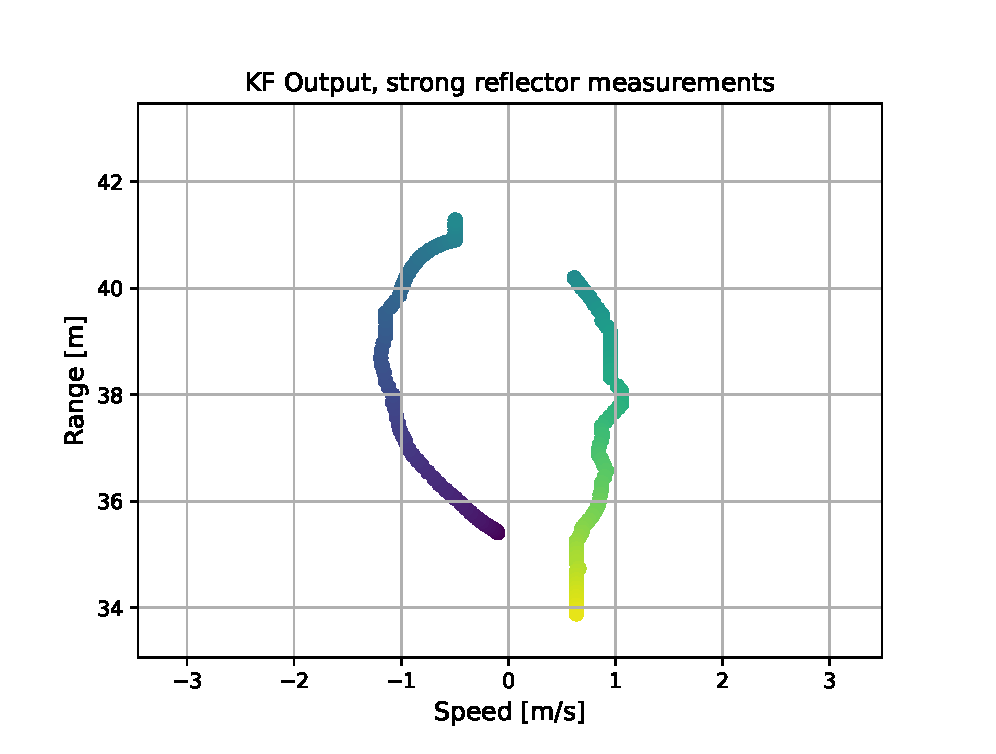
\includegraphics[width=0.7\textwidth]{Images/Test1/kf_track.eps}
	\caption{\small KF track of the target in the range/speed plane. Track is interrupted when the target stops and changes direction.}
	\label{fig:Test1_kf_track_strong_ref}
\end{figure}


\subsection{Human target detection}

The detection rate for measurements with a walking actor was compared for the various frame processing strategies presented in chapter \ref{chap:TDD pattern of the OFDM frame}. To increase time-aperture, subsequent frames were combined, and the observation time window stride was set to be lower than the number 
of concatenated frames, allowing for more updates through the measurement.
Clutter removal was performed to ensure precise estimation of the expected target position in NLOS conditions. 
CRAP has showed to outperform ECA-C in previously investigated LOS scenarios due to its ability to isolate static targets and better separate them \cite{Henninger_CRAP_2023}.
In NLOS both algorithms were tested as the information about static targets, lost with ECA-C, is anyway discarded.
Detection rate was obtained by using CRAP for the \gls{los} region, and compared for the two approaches in \gls{nlos}.
After obtaining the periodogram target returns are detected by using the range-adjusted exponential threshold presented in Section \ref{sec:radar_search_detection}.
Comparison of a sample radar update after CRAP and ECA-C is shown in Figure \ref{fig:Test1_huma_crap-ecac}.

	\begin{figure}[H]
	\centering
	
	\subfloat[Periodogram after applying CRAP.\label{fig:Test1_mhuman_crap}]{%
		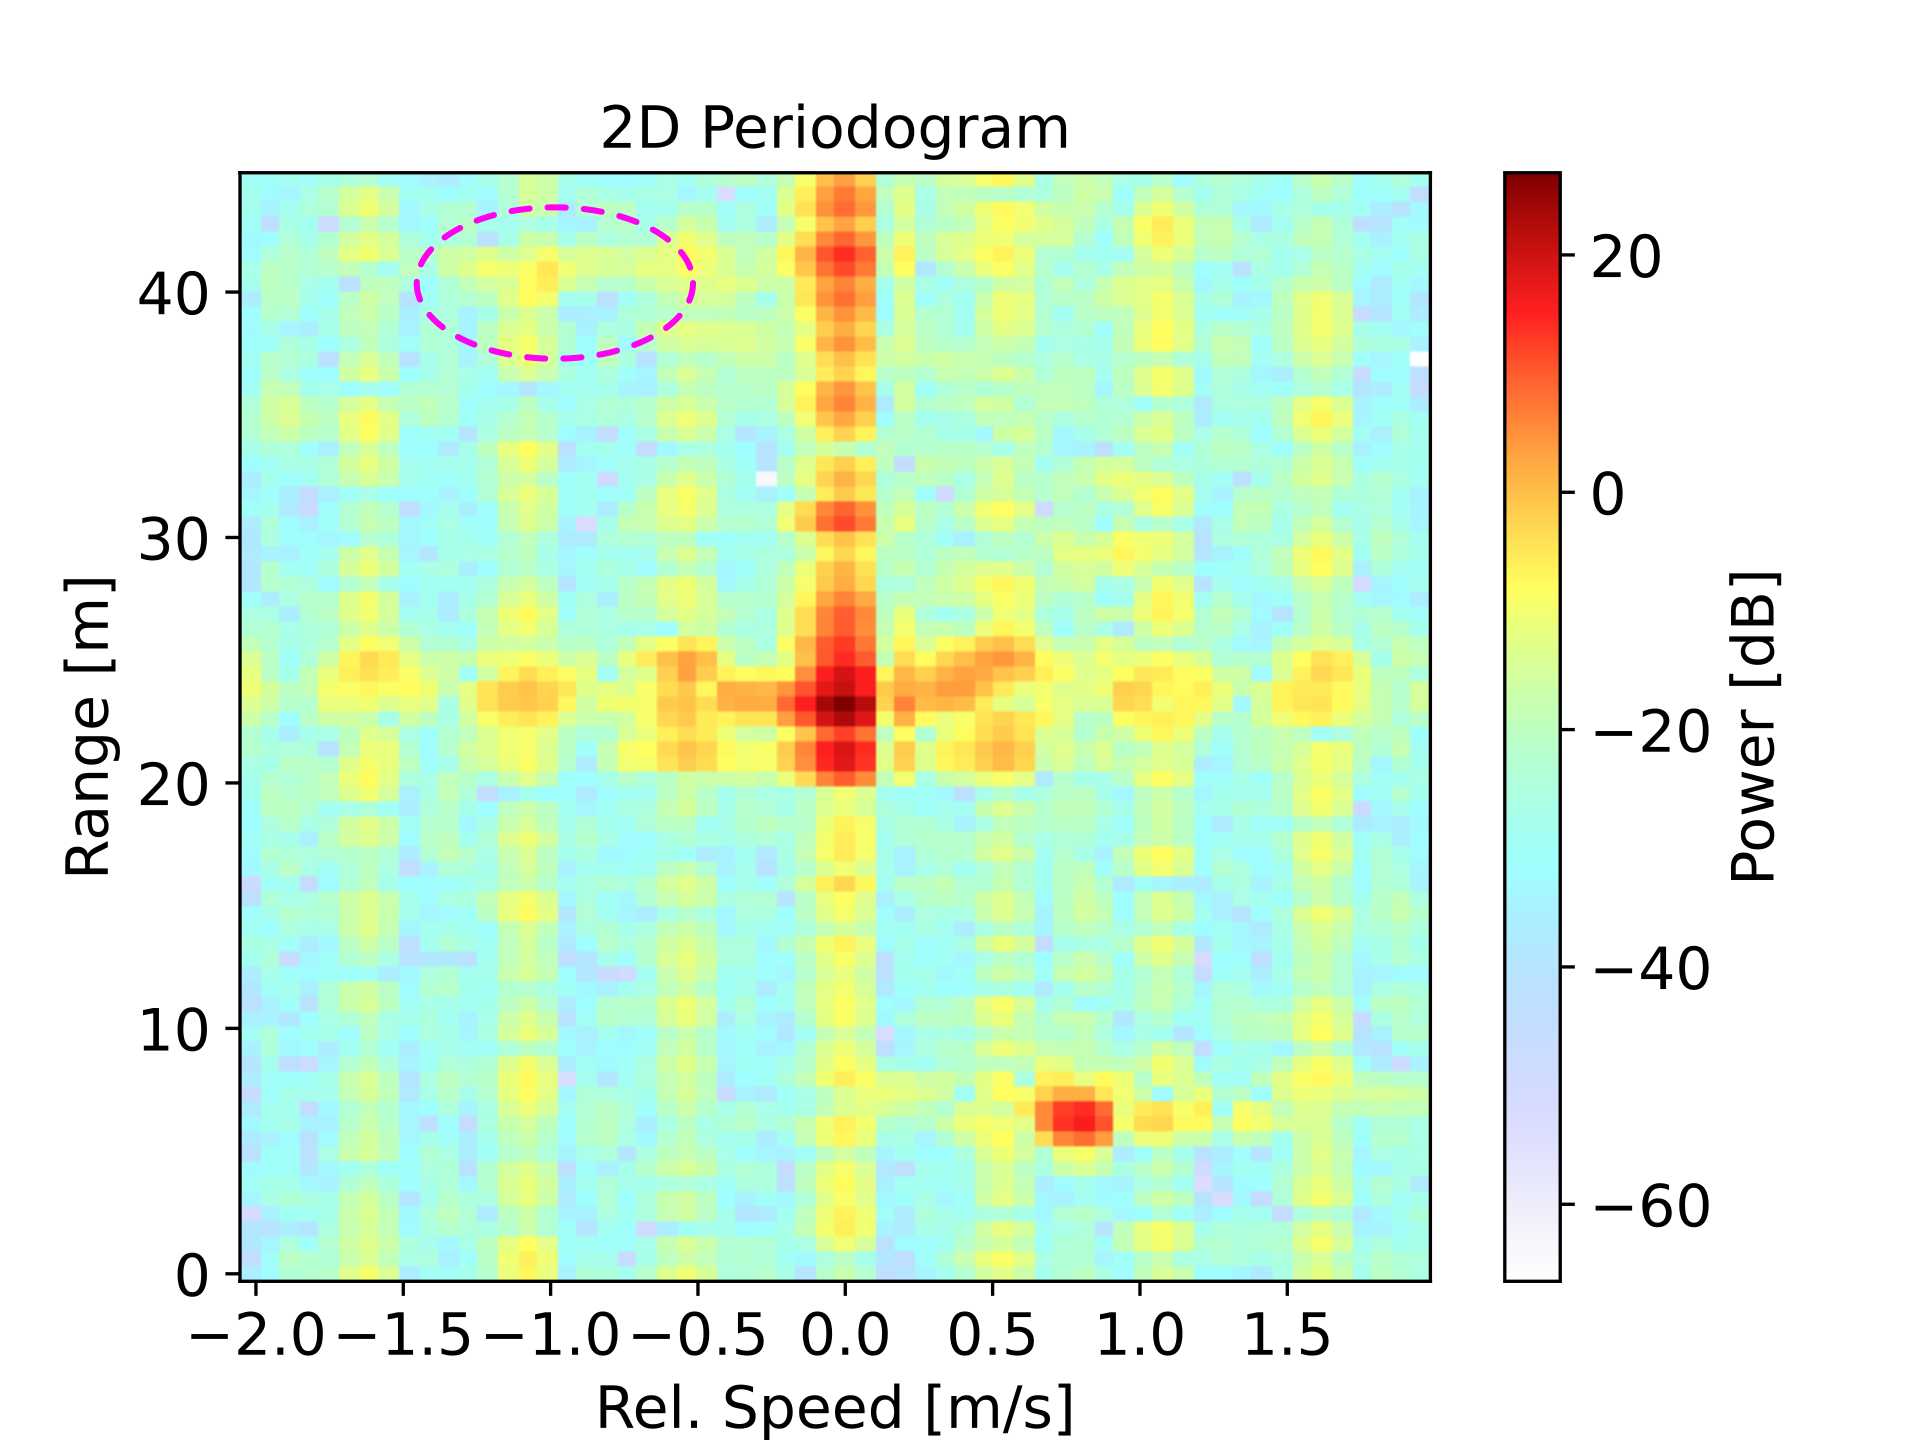
\includegraphics[scale=0.45]{Images/Test1/Human_crap_ecac/crap_labelled.png}%
	}\hfill
	\subfloat[Periodogram after applying ECA-C.\label{fig:Test1_mhuman_ecac}]{%
		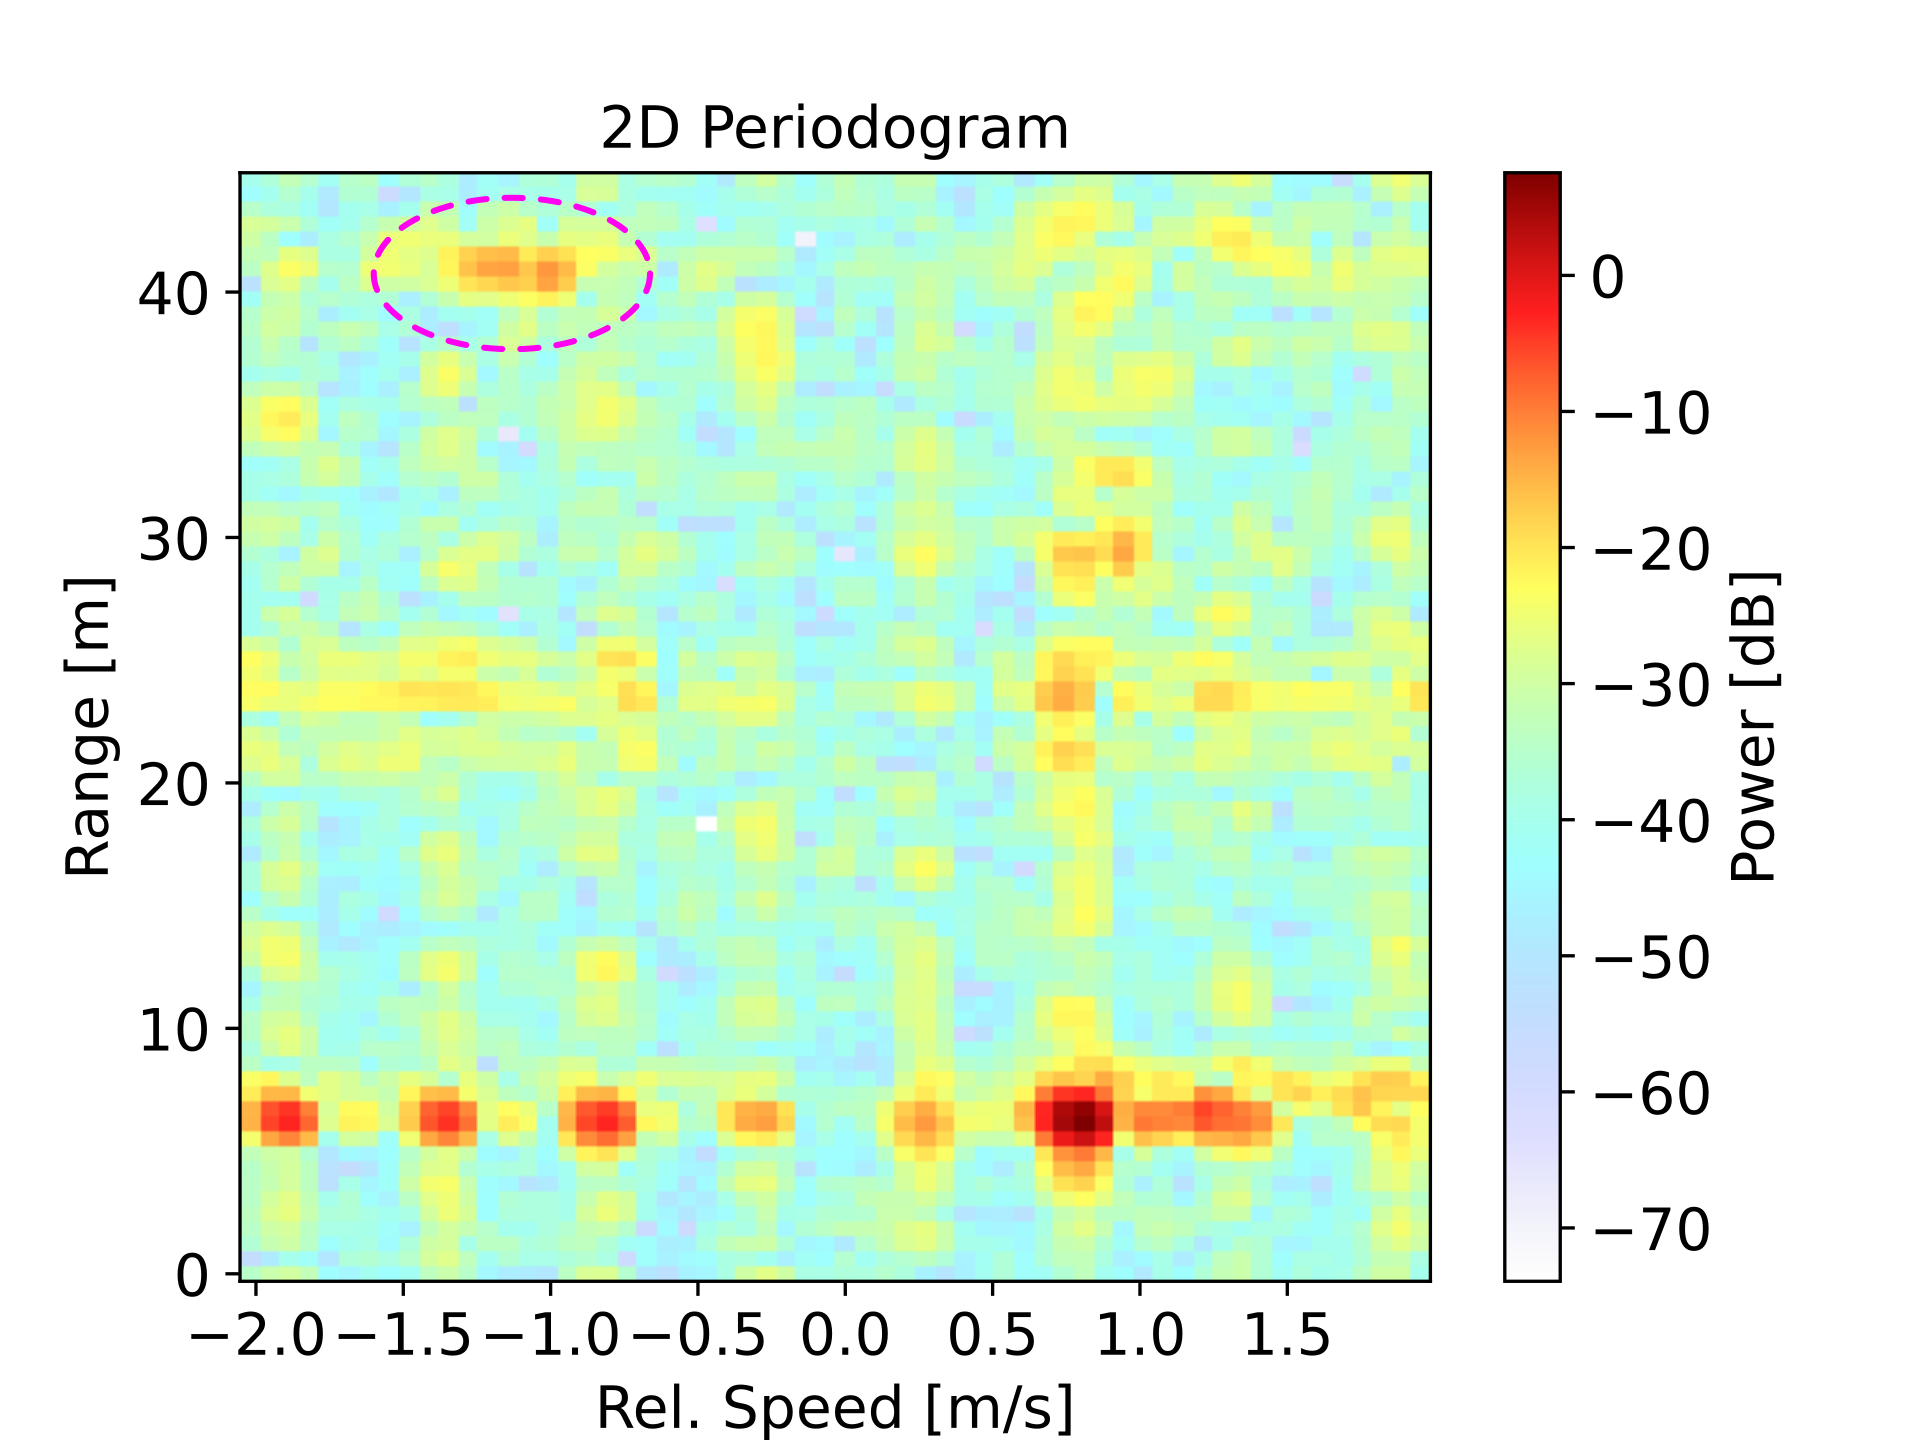
\includegraphics[scale=0.45]{Images/Test1/Human_crap_ecac/ecac_labelled.png}%
	}
	\caption[]{\small Comparison of periodograms from sensing acquisitions obtained in NOKIA's industrial test facility.
		Periodogram obtained by processing 6 consecutive frames.
		In \subref{fig:Test1_mhuman_crap} the NLOS return presents a single, but its power is comparable with the one of the nearby artefacts. In \subref{fig:Test1_mhuman_ecac} the NLOS return is enhanced, however the sidelobes of the LOS component are enhanced and its peak is slightly shifted.}
	\label{fig:Test1_huma_crap-ecac}
\end{figure}




Detection rate was estimated for the \textit{n}-strongest returns in \gls{nlos}, comparing them with the \gls{los} component.
The measured detection rate for various \gls{csi} decimation strategies are shown in Figure \ref{fig:Test1_detect_hist}. A larger time aperture resulted in better performance and higher detection probability.

\begin{figure}[H]
	\centering
	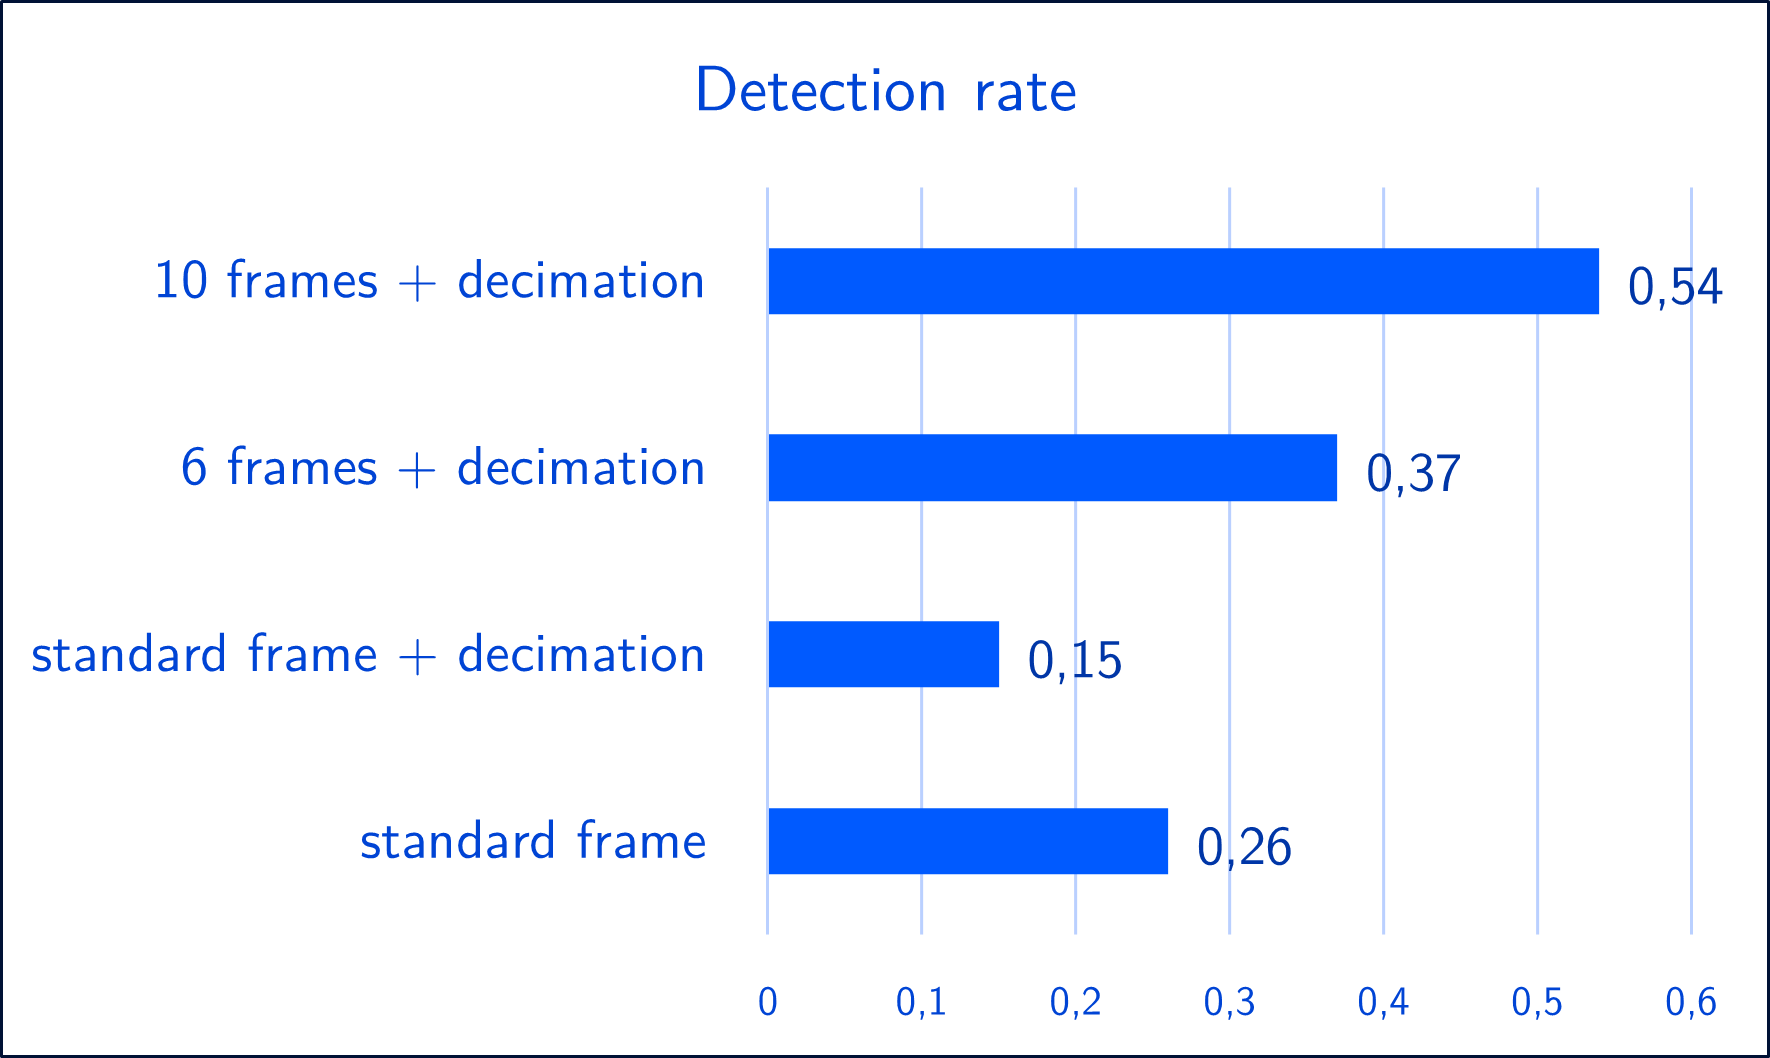
\includegraphics[width=0.7\textwidth]{Images/Test1/detect_hist/detect_hist_human_LMsans.png}
	\caption{Detection rate observed for human target in mixed LOS/NLOS measurement. Clutter removal performed with CRAP.}
	\label{fig:Test1_detect_hist}
\end{figure}

Increasing the time-aperture significantly improved the detection rate due to the larger \gls{snr}.

In most cases, the NLOS target return was not the strongest due to lower peak power compared to noise. Additionally, when increasing the time aperture, spectral artefacts were present.
Target returns occasionally suffered from channel fading, causing their power to change between consecutive updates. In contrast, artefacts' power remained relatively constant and proportional to the number of processed frames.

The detection rate was observed throughout the entire measurement, including frames where the target changed direction and was either static or presented a low-speed component. However, processing these time instants may have masked the NLOS component with clutter and resulted in a negative detection. Therefore, the effective detection rate, which is measured only when the target is in motion, is likely to be higher.


%TODO: change subsection title



% TODO: change picture with higher resolution one, maybe solved
%\begin{figure}[H]
%	\centering
%	%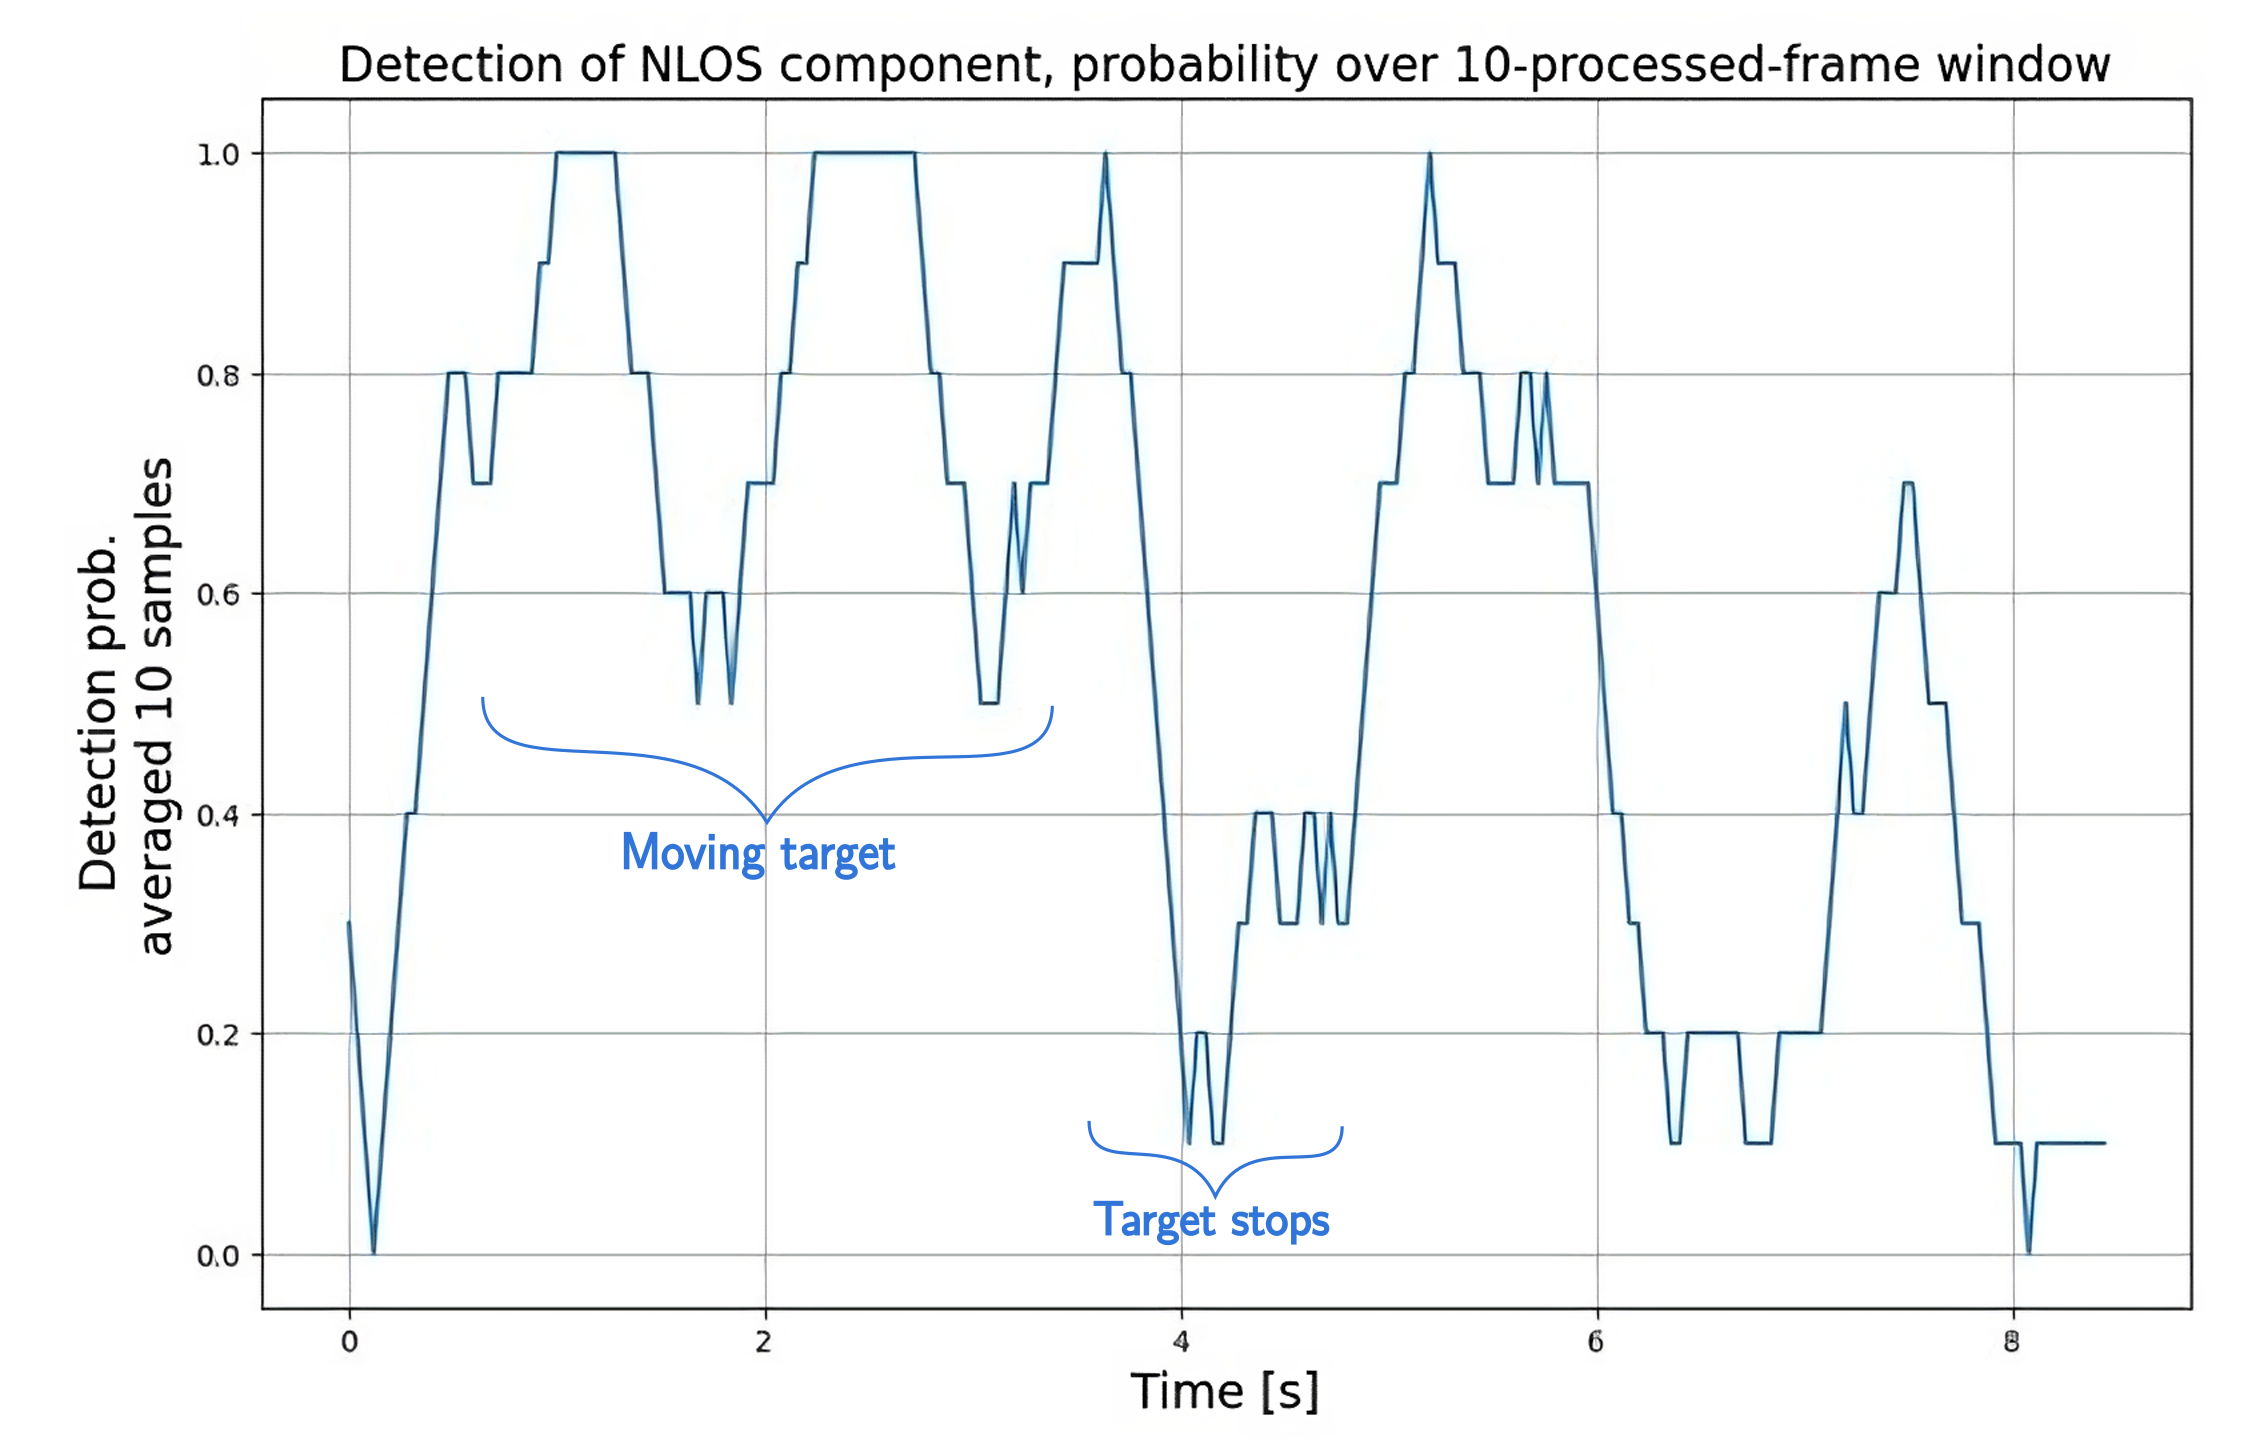
\includegraphics[width=0.7\textwidth]{Images/Test1/moving_avg-transformed_wtext}
%	\caption{Detection rate observed for human target in mixed LOS/NLOS measurement.}
%	\label{fig:Test1_moving_avg}
%\end{figure}


\subsubsection{Detection rate with separate clutter removal for NLOS}

CRAP is ideal for \gls{los} targets, while the power of the \gls{nlos} return is reduced to a level similar to the Doppler artefacts.
On the other hand, ECA-C introduces distortion and loss of information at zero speed, which is not suitable for any use case requiring \gls{los}, while it is able to enhance the power in the return compared to artifacts. In \gls{nlos} the static bin of the periodogram is discarded anyway, while for intrusion detection scenarios the interest lies in detecting targets while avoiding false positives rather than tracking and positioning said targets.
The detection rate was tested using separately CRAP and ECA-C for the LOS and NLOS regions, respectively. Figure \ref{fig:Test1_detect_hist_crap-ecac} shows the obtained detection rate, which shows improved performance.
\begin{figure}[H]
	\centering
	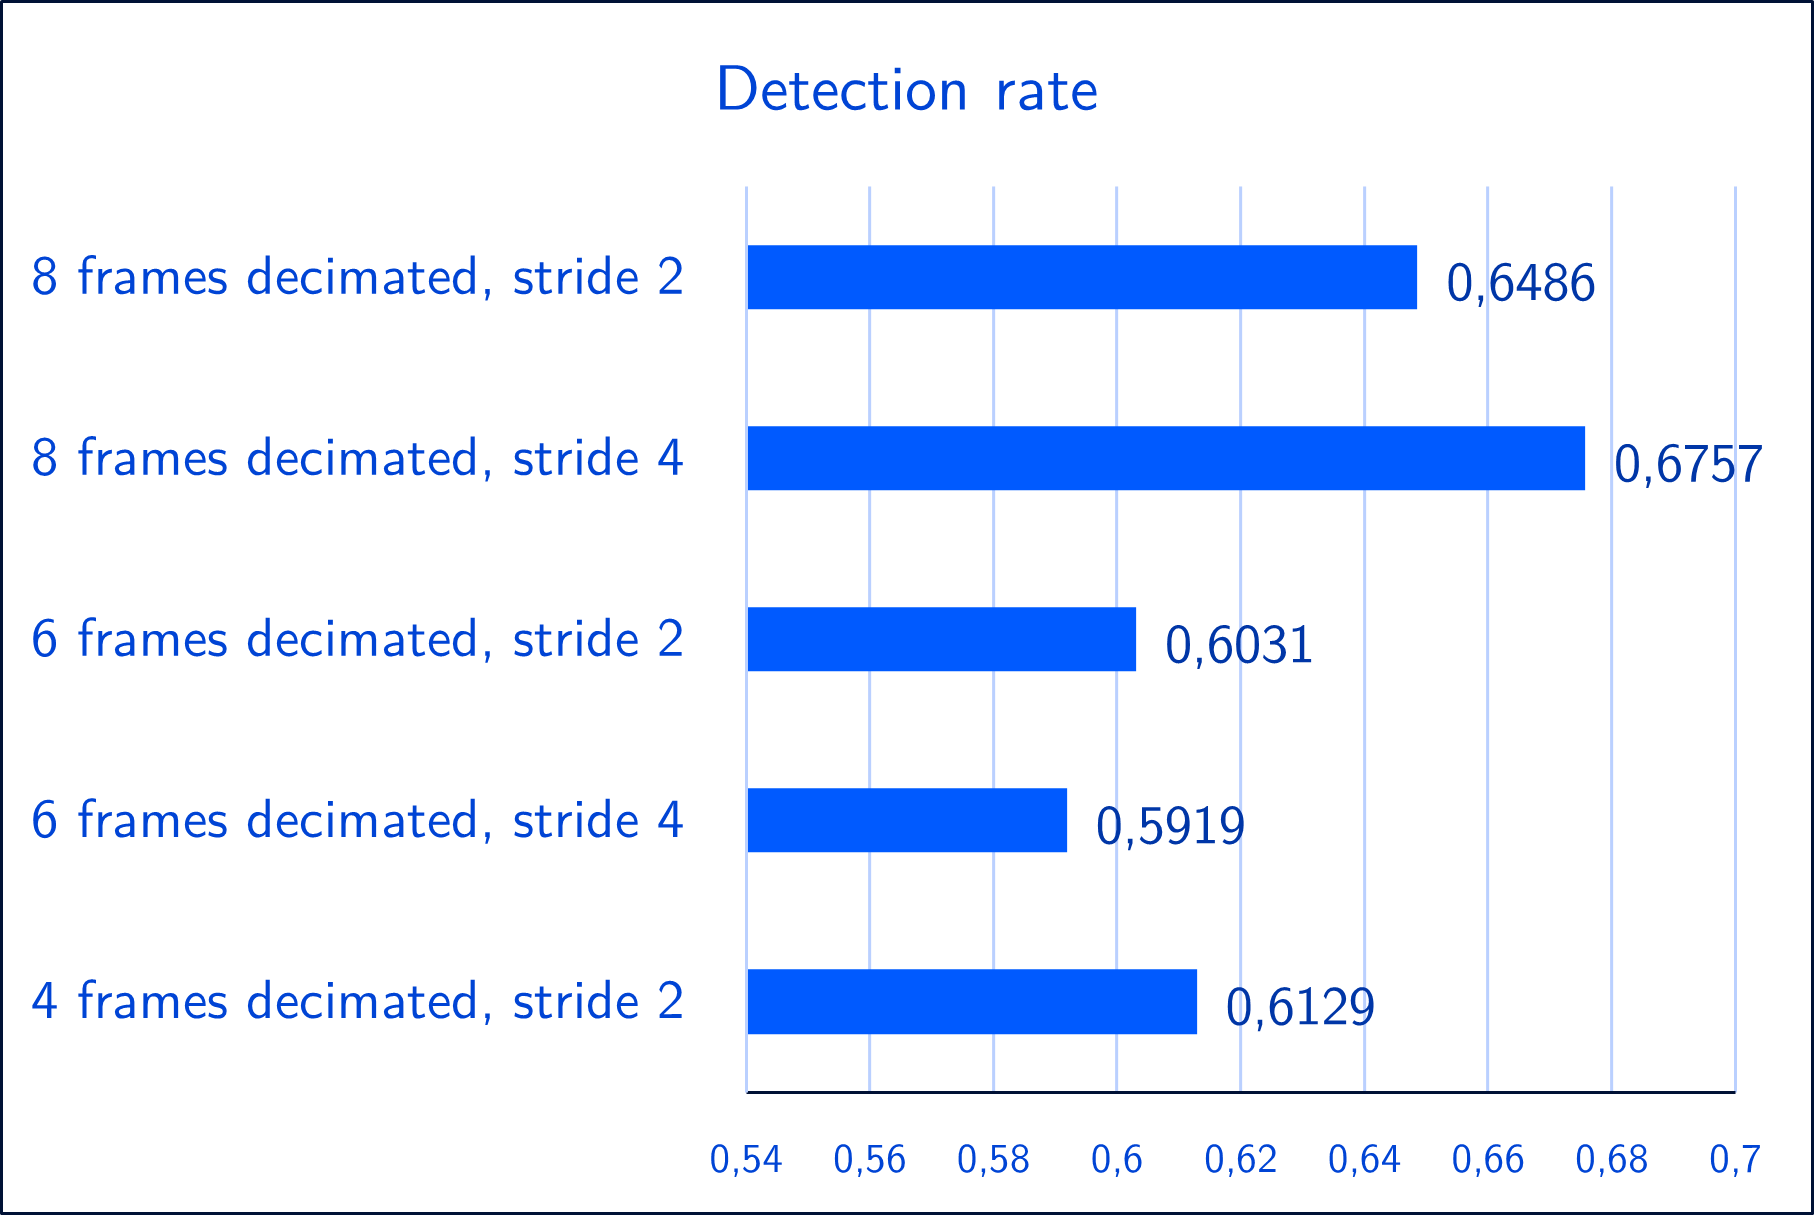
\includegraphics[width=0.7\textwidth]{Images/Test1/detect_hist/detect_hist_human_ECAC_LMsans.png}
	\caption{\small Detection rate observed for human target in mixed LOS/NLOS measurement. Clutter removal performed with ECA-C for the NLOS region and CRAP for the LOS.}
	\label{fig:Test1_detect_hist_crap-ecac}
\end{figure}
The measurement was not affected by the loss of information due to ECA-C when the target was static, as the bins of the periodogram corresponding to null speed were discarded regardless.


\subsection{Moving average of detection rate}

With the focus on intrusion detection, it is sufficient to detect the presence of the intruder once and raise an alarm accordingly.
A possible approach for discriminating the presence of actual targets from false alarms is to verify that \gls{nlos} peaks are continuously detected within a window of consecutive updates.
The sustained presence of the \gls{nlos} return over an observation window can be evaluated by computing the moving average of the detection rate over time.
Figure \ref{fig:Test1_detect_mov_avg} depicts the detection rate evaluated over a 0.5 s time window across the measurement, when applying ECA-C for the NLOS region and CRAP for the LOS one.
The calculation of the detection rate includes the parts of the measurements where the target stopped and changed direction (highlighted in red in Figure \ref{fig:Test1_detect_mov_avg}).
In these instances detection is negative, since no \gls{nlos} component is detected, as the bins of the periodogram corresponding to zero speed are discarded.
Nonetheless it can be observed that when the target is moving (\eg blue highlighted interval) its return is detected in most updates.
Although the measurement was conducted in a controlled, single-target scenario, these results open up the possibility of achieving true \gls{nlos} target detection.

\begin{figure}[H]
	\centering
	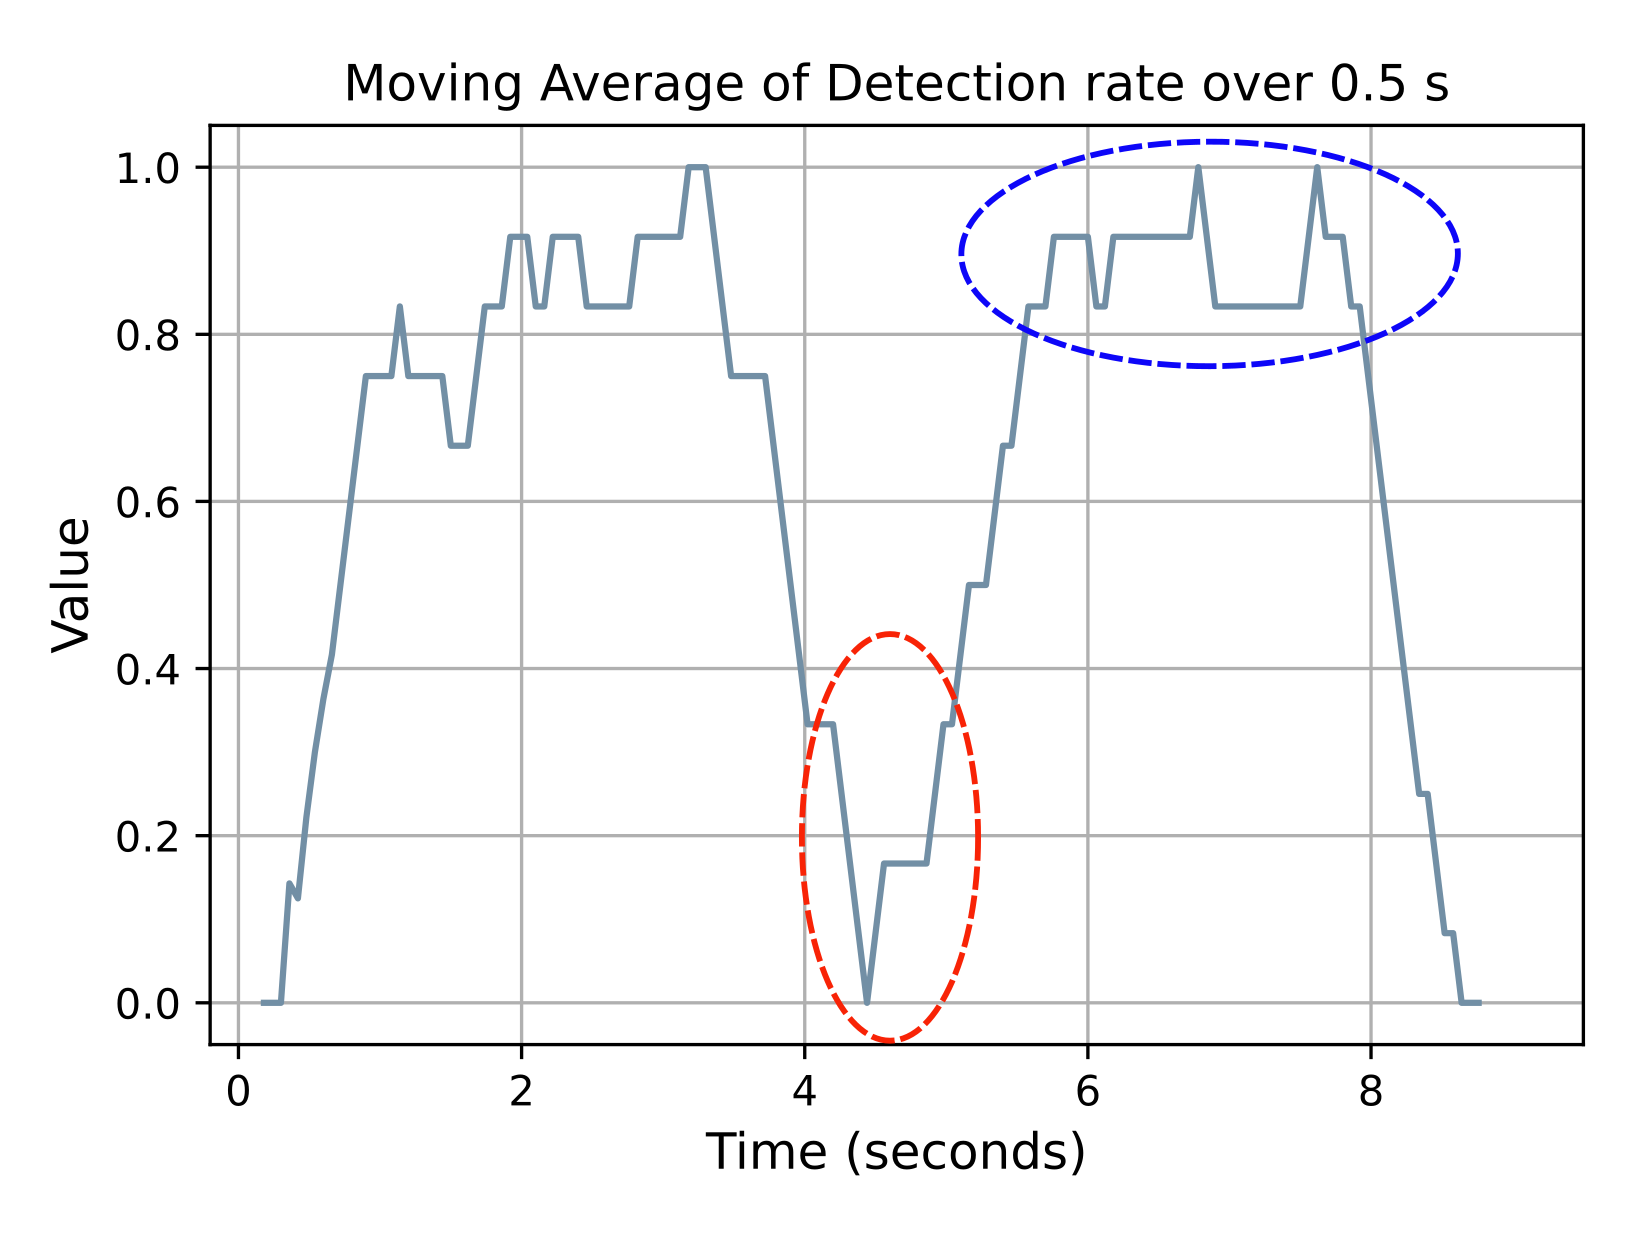
\includegraphics[width=0.7\textwidth]{Images/exec_specific/detect_mov_avg_bluepoli_highlighted.png}
	\caption{\small Detection rate observed for human target in mixed LOS/NLOS measurement. Clutter removal performed with ECA-C for the NLOS region and CRAP for the LOS.}
	\label{fig:Test1_detect_mov_avg}
\end{figure}
